\section{Streuungsmaße}
Um eine Verteilung sinnvoll beschreiben zu können sind zusätzlich zu den Lagemaßen noch Aussagen über die Streuung der Daten um das Mittel nötig.

\begin{definition}{Streuungsmaß}
	Ein \emph{Streuungsmaß} ist eine Abbildung $S:\R^n\rightarrow \R$ für die gilt
	\begin{equation*}
		S(x_1+a,\ldots,x_n+a)=S(x_1,\ldots,x_n) \quad\forall a,x_i\in\R (1\leq i\leq n)
	\end{equation*}
	Ein Streuungsmaß stellt dar, wie weit gestreut Werte einer Verteilung um ein Mittel liegen.
\end{definition}

\subsection{Spannweite, Stichprobenspannweite}
Die Stichproblenspannweite stellt dar, in welchem Bereich die Ausprägungen liegen, denn diese ist einfach
\begin{equation*}
	x_{\operatorname{max}}-x_{\operatorname{min}}.
\end{equation*}


\subsection{Mittlere absolute Abweichung vom Median}
Die mittlere absolute Abweichung vom Median stellt eine robustere Alternative zur Stichprobenvarianz dar. Sie ist für eine Urliste $U=\simpleset{x_1,\ldots,x_n}$ definiert als 
\begin{equation*}
	\frac 1n\sum_{i=1}^n|x_i-x_{\operatorname{med}}|
\end{equation*}


\subsection{Quantile}
Ein Quantil ist eine Kennzahl, die Daten nach einer relativen Häufigkeit trennt. So trennt das $p$-Quantil einer Verteilung die Daten som dass etwa $p*100\%$ der Daten darunter und $(1-p)*100\%$ darüber liegen. Damit ist der Median gerade das $50\%$-Quantil.

\begin{definition}{Quantile}
	Sei $U=\simpleset{x_1,\ldots,x_n}$ eine geordnete Urliste, d.h. $x_1\leq\ldots\leq x_j\leq\ldots\leq x_n$. Das $p$-Quantil $x_p$ ist eine Ausprägung $x_p\in U$ für die gilt
	\begin{equation*}
		\frac{\left|\set{i\in\N}{x_i\leq x_p, x_i\in U}\right|}{n}\geq p \text{ und } \frac{\left|\set{i\in\N}{x_i\geq x_p, x_i\in U}\right|}{n}\geq 1-p
	\end{equation*}
	Das heißt es liegen $p\%$ der Daten unterhalb und $(1-p)\%$ der Daten oberhalb des $p$-Quantils.

	Sinnvoll berechnen lässt sich das $p$-Quantil durch die Formel
	\begin{equation*}
		x_p=\begin{cases}
			\frac12(x_{(n*p)}+x_{(n*p+1)}) &\text{, falls $n*p$ ganzzahlig}\\
			x_{(\lfloor n*p\rfloor)+1} &\text{ sonst}
		\end{cases}
	\end{equation*}
\end{definition}
Dabei nennt man das $25\%$-Quantil auch das \emph{untere Quartil} und entsprechend das $75\%$-Quantil das \emph{obere Quartil}.

\begin{definition}{Interquartilsabstand}
	Für metrische Merkamel ist der sogenannte \emph{Interquartilsabstand (interquartile range)} die Distanz
	\begin{equation*}
		d_Q=\operatorname{IQR}=x_{0.75}-x_{0.25}.
	\end{equation*}
	Der IQR wird zum Beispiel beim Box-Plot verwendet. 
\end{definition}
Mit dem IQR können Zäune festgelegt werden, außerhalb derer sich höchstwahrscheinlich Ausreißer des Merkmals befinden. Ein Beispiel hierfür ist zum Beispiel der untere Zaun $z_u=x_{0.25}-1.5*d_Q$ und entsprechend die Obergrenze $z_o=x_{0.75}+1.5*d_q$, diese Werte werden wiederum beim Box-Plot verwendet.

\subsection{Fünf-Punkte-Zusammenfassung}
Die Quartile, das Minimum, Maximum sowie der Median teilen den Datensatz in vier Teile, wobei jeder etwa ein Viertel der Merkmale enthält. Die Angabe dieser fünf Werte wird auch als Fünf-Punkte-Zusammenfassung bezeichnet.

\subsubsection{Box-Plot}
Das Box-Plot ist eine einfache Art und Weise die Ausprägungen einer Verteilung zu visualisieren. Für den Box-Plot wird eine fünf-Punkte-Zusammenfassung, $(z_u, x_{0.25}, x_{\operatorname{med}}, x_{0.75}, z_o)$ verwendet, wobei $z_u$ und $z_o$ beim modifizierten Box-Plot von der klassischen fünf-Punkte-Zusammenfassung abweichen können.
Daran werden zwei Definitionen unterschieden, der \glqq normale\grqq\ und der modifizierte Box-Plot.

Beim Box-Plot wird ein Rechteck zwischen den Quartilen gezeichnet, das $x_{\operatorname{med}}$ eingezeichnet als Linie oder Punkt beinhaltet.
So sieht man dass sich $50\%$ der Datenpunkte innerhalb der Box befinden. Die nach außen gezeichneten Linien geben an, wie weit die restlichen $50\%$ der Datenpunkte gestreut liegen. Diese sogenannten Whiskers enden in Abhängigkeit von $z_u$ bzw. $z_o$, diese Werte unterscheiden sich bei den beiden Definitionen.

\paragraph{Normaler Box-Plot}
Das Fünftupel besteht aus den Werten $(x_{\operatorname{min}}, x_{0.25}, x_{\operatorname{med}}, x_{0.75}, x_{\operatorname{max}})$. Wobei $x_{\operatorname{min}}$ und $x_{\operatorname{max}}$ die kleinste und größte Ausprägung der Verteilung darstellen. So sind alle Werte in der Spannweite der Whiskers enthalten. Ein Box-Plot sieht dann wie folgt aus

\begin{center}
	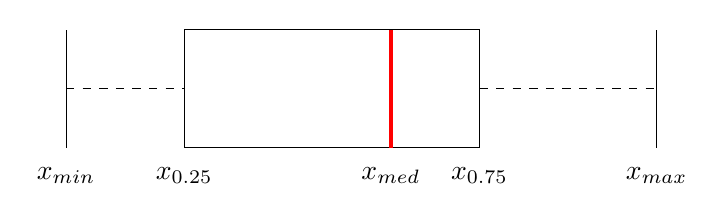
\begin{tikzpicture}[scale=0.75]
		\draw[black] (0,0) rectangle (5,2);
		\draw[black, dashed] (-2, 1) to (0,1) (5,1) to (8,1);
		\draw[black] (-2,0) to (-2,2) (8,0) to (8,2);
		\draw[red, line width=0.5mm] (3.5,0) to (3.5,2);

		\draw (-2,0) node[label={below:$x_{\operatorname{min}}$}] {};
		\draw (0,0) node[label={below:$x_{0.25}$}] {};
		\draw (3.5,0) node[label={below:$x_{\operatorname{med}}$}] {};
		\draw (5,0) node[label={below:$x_{0.75}$}] {};
		\draw (8,0) node[label={below:$x_{\operatorname{max}}$}] {};
	\end{tikzpicture}
\end{center}


\paragraph{Modifizierter Box-Plot (nach Fahrmeir)}
Der wichtigste Unterschied zum normalen Box-Plot ist dass, anstatt der minimalen und maximalen Werte für $z_u, z_o$ ein Zaun gewählt wurde. So ist $z_u=x_{0.25}-1.5*d_Q$ und $z_o=x_{0.75}+1.5*d_Q$ wobei $d_Q$ der Interquartilsabstand ist. Allerdings ist zu beachten dass die Whiskers von der größten/ kleinsten Ausprägung innerhalb des Zauns zur Box ausgehen. Liegen also beispielweise innerhalb des Bereichs $[z_u,x_{0.25}]$ keine Datenwerte, so existiert kein unterer Whisker. Datenpunkte, die außerhalb des Zauns liegen, werden mit Punkten dargestellt. Dies ist ein gutes Anzeichen für eventuelle Ausreißer.

\begin{center}
	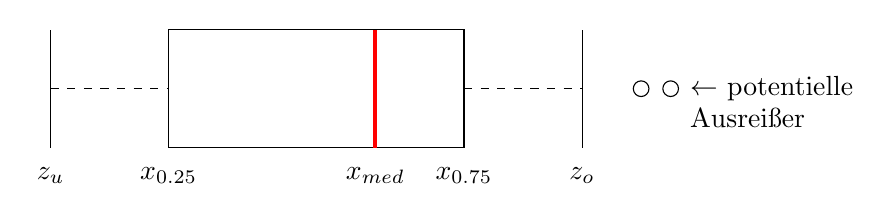
\begin{tikzpicture}[scale=0.75]
		\draw[black] (0,0) rectangle (5,2);
		\draw[black, dashed] (-2, 1) to (0,1) (5,1) to (7,1);
		\draw[black] (-2,0) to (-2,2) (7,0) to (7,2);
		\draw[red, line width=0.5mm] (3.5,0) to (3.5,2);

		\draw (-2,0) node[label={below:$z_u$}] {};
		\draw (0,0) node[label={below:$x_{0.25}$}] {};
		\draw (3.5,0) node[label={below:$x_{\operatorname{med}}$}] {};
		\draw (5,0) node[label={below:$x_{0.75}$}] {};
		\draw (7,0) node[label={below:$z_o$}] {};
		\draw (8,1) node[draw=black, fill=white, circle, inner sep=2pt] {};
		\draw (8.5,1) node[draw=black, fill=white, circle, inner sep=2pt] {};
		\draw (8.5,1) node[label={right:$\leftarrow$\ potentielle}] {};
		\draw (8.5,0.5) node[label={right:Ausreißer}] {};
	\end{tikzpicture}
\end{center}


\subsection{Standardabweichung}
Die Standardabweichung ist für eine Urliste $U=\simpleset{x_1,\ldots,x_n}$ von metrischen Daten definiert als
\begin{equation*}
	\tilde s=\sqrt{\frac 1n\sum_{i=1}^n (x_i-\overline x)^2}=\sqrt{\sum_{i=1}^n (a_i-\overline x)^2*f_i}
\end{equation*}
wobei die $a_i$ die Ausprägungen der Urliste sind und $f_i$ die relative Häufigkeit der Ausprägung $a_i$ ist.

Unter einer linearen Transformation $x\mapsto ax+b$ der Ausprägungen wird $\tilde s$ um $|a|$ gedehnt. Eine Verschiebung der Werte um $b$ hat keine Auswirkung.

\subsection{Variationskoeffizient}
Der Variationskoeffizient ist eine maßstabsunabhängige Maßzahl für die Streuung, sie basiert auf der Standardabweichung und ist definiert als
\begin{equation*}
	v=\frac{\tilde s}{\overline x},\quad \overline x>0
\end{equation*}

\subsection{Varianz, empirische Varianz}
Die empirische Varianz ist das Quadrat der Standardabweichung $\tilde s^2$.
\begin{equation*}
	\tilde s^2 = \frac 1n\sum_{i=1}^n (x_i-\overline x)^2
\end{equation*}
Sowohl Standardabweichung als auch die Varianz sind nicht resistent, reagieren also sehr empfindlich auf Ausreißer. 

Für eine Berechnung von Hand gilt der sogenannte Verschiebungssatz
\begin{satz}{Verschiebungssatz}
	Für jedes $c\in\R$ gilt
	\begin{equation*}
	    \sum_{i=1}^n(x_i-c)^2=\sum_{i=1}^n(x_i-\overline x)^2+n(\overline x -c)^2.
	\end{equation*}
	Damit gilt insbesondere mit $c=0$ für die Varianz
	\begin{equation*}
		\tilde s^2=\left(\frac1n \sum_{i=1}^n x_i^2\right)-\overline x.
	\end{equation*}
\end{satz}
\paragraph{Beweis:}
\begin{align*}
    \sum_{i=1}^n(x_i-c)^2&=\sum_{i=1}^n(x_i-\overline x+\overline x-c)^2\\
    &=\sum_{i=1}^n\left[(x_i-\overline x)^2+2(x_i-\overline x)(\overline x-c)+(\overline x-c)^2\right]\\
    &=\sum_{i=1}^n(x_i-\overline x)^2 + \underbrace{2(\overline x-c)\sum_{i=1}^n(x_i-\overline x)}_{=0}+\sum_{i=1}^n(\overline x-c)^2\\
    &=\sum_{i=1}^n(x_i-\overline x)^2+n(\overline x -c)^2
\end{align*}

\paragraph{Lineare Transformation}
Mit einer linearen Abbildung der Ausprägungen $y_i=ax_i+b$ verhält sich die Varianz der Daten $y_i$
\begin{equation*}
	\tilde s_y^2=a^2\tilde s_x^2\text{ bzw. }\tilde s_y=|a|\tilde s_x
\end{equation*}
dies ergibt sich direkt aus den Formeln für die Varianz
\begin{align*}
    \tilde s_y^2&=\frac 1n\sum_{i=1}^n(y_i-\overline y)^2\\
    &=\frac 1n \sum_{i=1}^n(ax_i+b-a\overline x-b)^2\\
    &=a^2\frac 1n\sum_{i=1}^n(x_i-\overline x)^2=a^2\tilde s_x^2
\end{align*}

\subsection{Stichprobenvarianz}
Die Stichprobenvarianz stellt ein nicht resistentes Streuungsmaß dar. Sie ist für eine Urliste $U=\simpleset{x_1,\ldots,x_n}$ definiert als
\begin{equation*}
	s^2=\frac{1}{n-1}\sum_{i=1}^n (x_i-\overline x)^2=\frac{1}{n-1}\sum_{i=1}^n x_i^2 - n*\overline x^2
\end{equation*}



\section{Konzentrationsmaße}
Konzentration geben Aufschluss über die Stärke der Konzentration von Daten.
\subsection{Lorenzkurve}
Ausgehend von geordneten Ausprägungen $x_1\leq\ldots\leq x_n$ stellt die Lorenzkurve den Anteil der kumulierten relativen Merkmalssumme bezüglich dem Anteil der Merkmalsträger von der Grundgesamtheit dar.

\begin{definition}{Lorenzkurve}
	Die Lorenzkurve ergibt sich als Streckenzug durch die Punkte $(0,0), (u_1,v_1),\ldots,(1,1)$ wobei
	\begin{align*}
	    u_j=\frac jn \quad \text{und}\quad 
	    v_j=\frac{\sum_{i=1}^j x_i}{\sum_{i=1}^n x_i}
	\end{align*}
ist.
\end{definition}

Der Grundgedanke ist, darzustellen auf welchen Teil der Merkmalsträger welcher Anteil der Merkmalssumme zuruckgeht.

Die Lorenzkurve wächst immer monoton und konvex, d.h. sie wölbt sich nach unten.

\subsection{Gini-Koeffizient}
In der Lorenzkurve drückt sich Konzentration der Daten durch Entfernung von der ersten Winkelhalbierenden aus. Genau dies nutzt der Gini-Koeffizient $G$ aus.

$G$ ist gleich dem Verhältnis zwischen dem von Lorenzkurve und Diagonale eingeschlossenen Flächeninhalt und der Fläche unter der Winkelhalbierenden.

\begin{equation*}
	G=\frac{2\sum_{i=1}^n ix_i}{n\sum_{i=1}^n x_i}-\frac{n+1}{n}\quad G\in[0,\infty)
\end{equation*}

Dabei ist der minimale Wert des Gini-Koeffizienten $G_{\text{min}}=0$ und das Maximum ist $G_{\text{max}}=\frac{n-1}n$.

Da der Wert des Gini-Koeffizienten mit von der Eingabegröße abhängnen kann, bietet sich der normierte Gini-Koeffizient für Vergleiche an
\begin{equation*}
	G^\ast = \frac{G}{G_{\text{max}}}=\frac{n}{n-1}G\quad G^\ast\in[0,1]
\end{equation*}
